\chapter{Osciladores Senoidales}
 \hspace{10pt} \textbf{Ejercicio 1}: Dado el  circuito y los diagramas de Bode de
la red de atenuación $\beta$ de la figura \ref{oscila1} , hallar
$R_x$ límite para que oscile. Obtener la frecuencia de oscilación.

\begin{figure}[h]
	\centering
	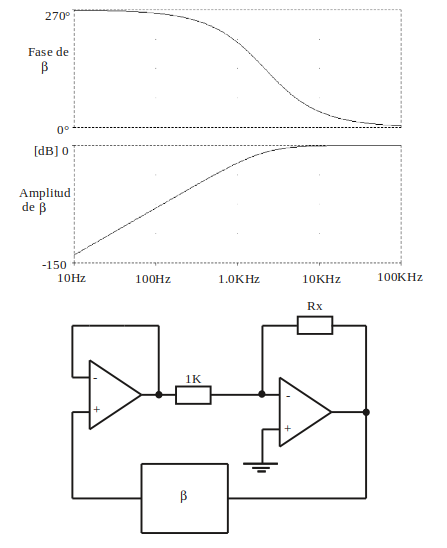
\includegraphics[width=0.6\linewidth]{figuras/oscila1.png}\\
	\caption{Ejercicio 1.}\label{oscila1}
\end{figure}


\textbf{Ejercicio 2}: En el circuito de la figura \ref{oscila2}
hallar el valor de R para que la frecuencia de oscilación sea de 475
Hz. Obtener el valor de $R_s$ para que se cumpla la condición de
amplitud.

\begin{figure}[h]
	\centering
	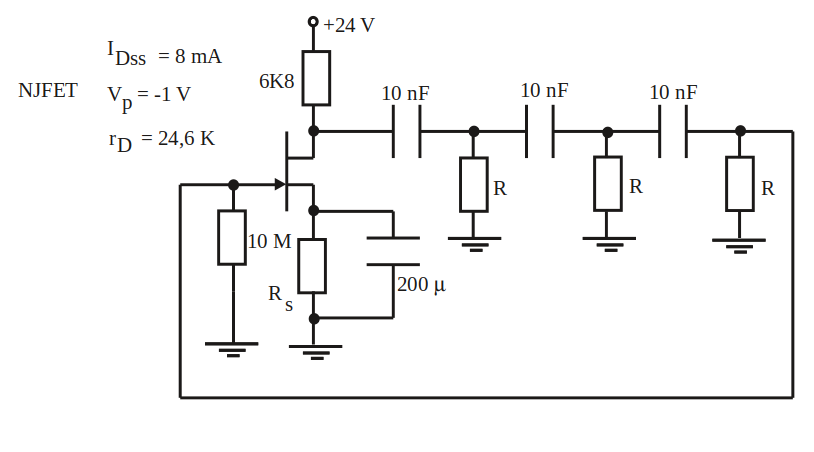
\includegraphics[width=0.8\linewidth]{figuras/oscila2.png}\\
	\caption{Ejercicio 2.}\label{oscila2}
\end{figure}

\textbf{Ejercicio 3}: Diseñe un oscilador por desplazamiento de fase
que genere una señal senoidal de $f = 2 KHz$ con $v_o =
1\widehat{\widehat{V}}$ de amplitud como mínimo sobre  una carga
$R_L = 470 \Omega$. Utilice el mínimo número de dispositivos activos
posible y trate que el diseño requiera un único ajuste.

\textbf{Ejercicio 4}: El circuito de la figura \ref{oscila4} es un
oscilador puente de Wien. a) Determinar las condiciones de
oscilación y las ventajas y desventajas frente al de desplazamiento
de fase (suponer llave S en posición 1). b) Graficar la
transferencia de la red de realimentación en función de la
frecuencia normalizada en $\frac{\displaystyle w}{\displaystyle
	w_o}$. c) Explicar el funcionamiento del control automático de
ganancia (llave S en posición 2). d) Calcular, en función del
amplificador operacional empleado, la máxima frecuencia de salida
sin distorsión.

\begin{figure}[h]
	\centering
	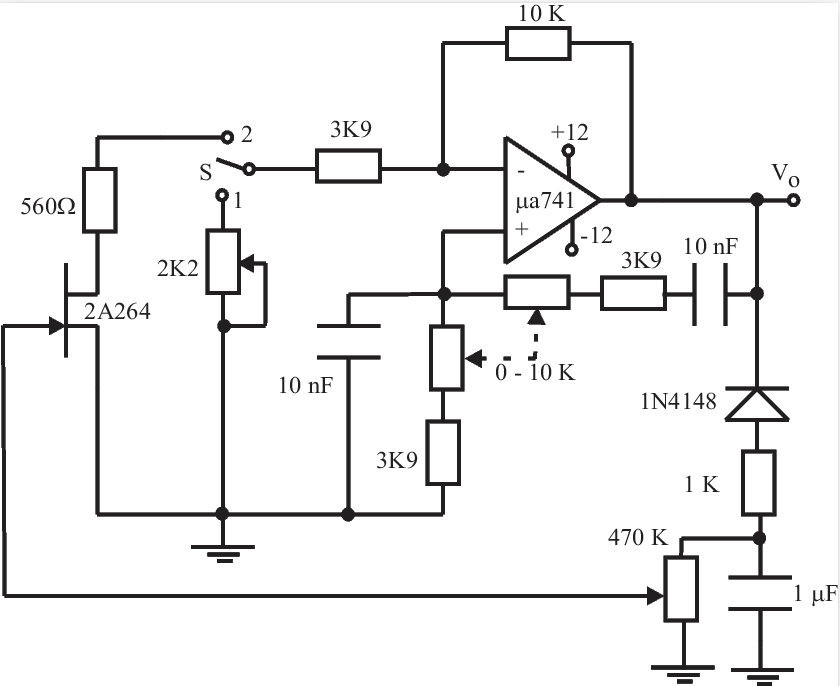
\includegraphics[width=0.6\linewidth]{figuras/oscila4ci.png}\\
	\caption{Ejercicio 4.}\label{oscila4}
\end{figure}


\textbf{Ejercicio 5:} Dado el circuito de la figura \ref{oscila5}:
adoptar un valor de $R_{C1}$ para que se cumpla la condición de
amplitud, con dicho valor calcular la frecuencia de oscilación.

\begin{figure}
	\centering
	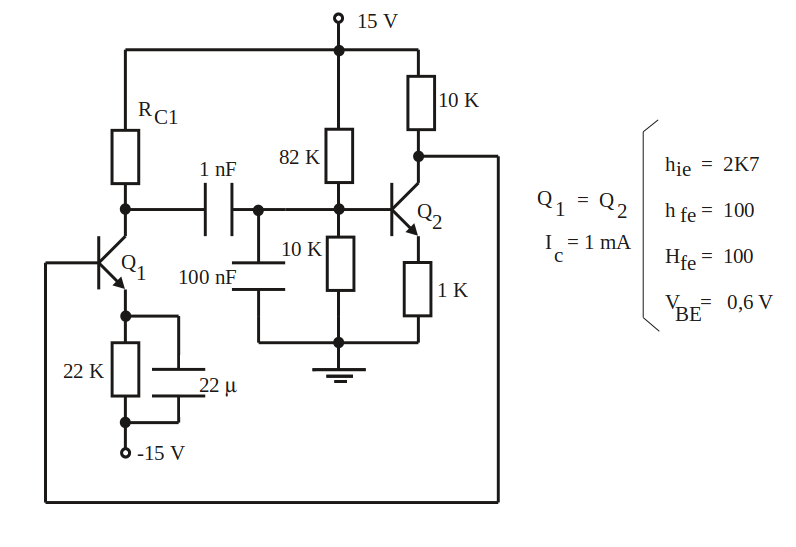
\includegraphics[width=0.6\linewidth]{figuras/oscila5.png}\\
	\caption{Ejercicio 5.}\label{oscila5}
\end{figure}

\textbf{Ejercicio 6}: ¿Qué valor debe tener $R_x$ para que se cumpla
la condición de amplitud?. ¿ Cuál será la frecuencia de oscilación?.
Ver figura \ref{oscila6}.

\begin{figure}
	\centering
	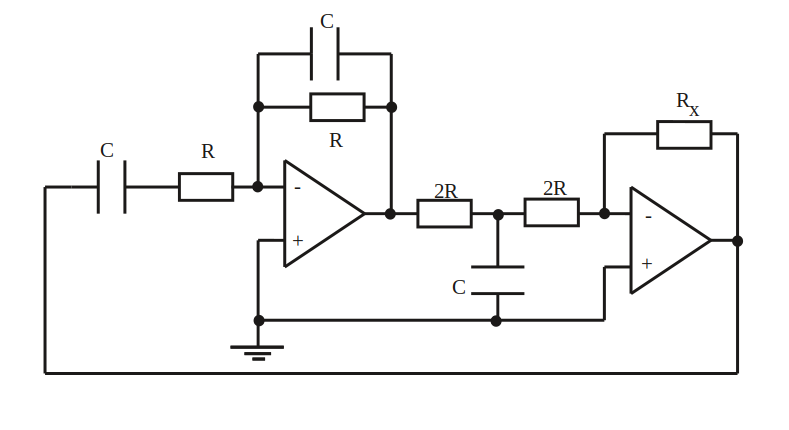
\includegraphics[width=0.6\linewidth]{figuras/oscila6.png}\\
	\caption{Ejercicio 6.}\label{oscila6}
\end{figure}

\textbf{Ejercicio 7}: Explicar el funcionamiento del oscilador de la
figura \ref{oscila7}. Hallar las condiciones de oscilación y la
frecuencia de la señal obtenida.

\begin{figure}
	\centering
	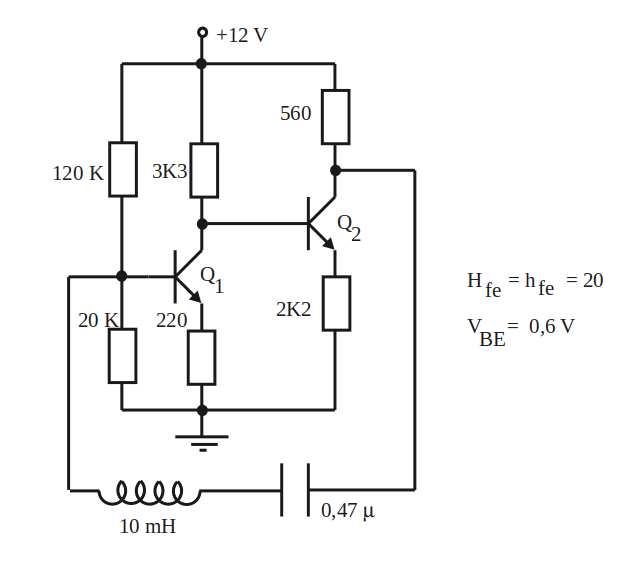
\includegraphics[width=0.6\linewidth]{figuras/oscila7.png}\\
	\caption{Ejercicio 7.}\label{oscila7}
\end{figure}

\textbf{Ejercicio 8}:  Diseñar un oscilador tipo Hartley y uno tipo
Colpits, ambos con una frecuencia de oscilación de 3 MHz, usando
como amplificador un TBJ 2A407 o un JFET 2A244.

\textbf{Ejercicio 9}: En el circuito de la figura \ref{oscila9}
obtener  la frecuencia de oscilación y estimar la estabilidad en
frecuencia.

\begin{figure}
	\centering
	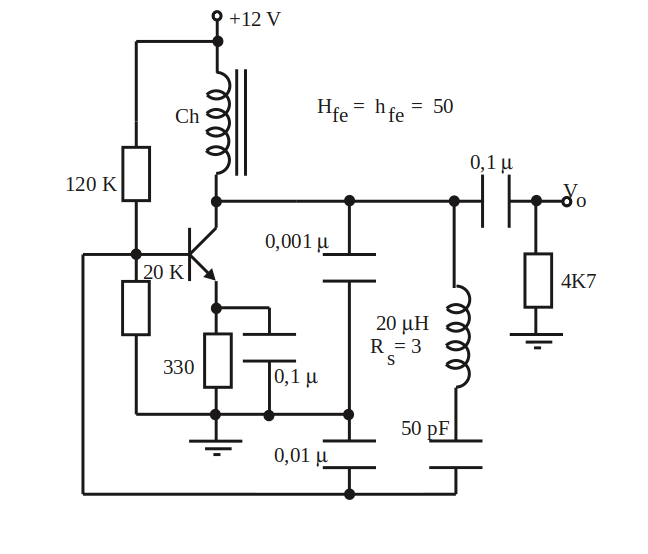
\includegraphics[width=0.8\linewidth]{figuras/oscila9.png}\\
	\caption{Ejercicio 9.}\label{oscila9}
\end{figure}

\textbf{Ejercicio 10}: En el oscilador de la figura \ref{oscila10},
calcular la frecuencia de oscilación, el $Q_C$ y el valor de
$I_{CQ}$ para que comiencen las oscilaciones.

\begin{figure}
	\centering
	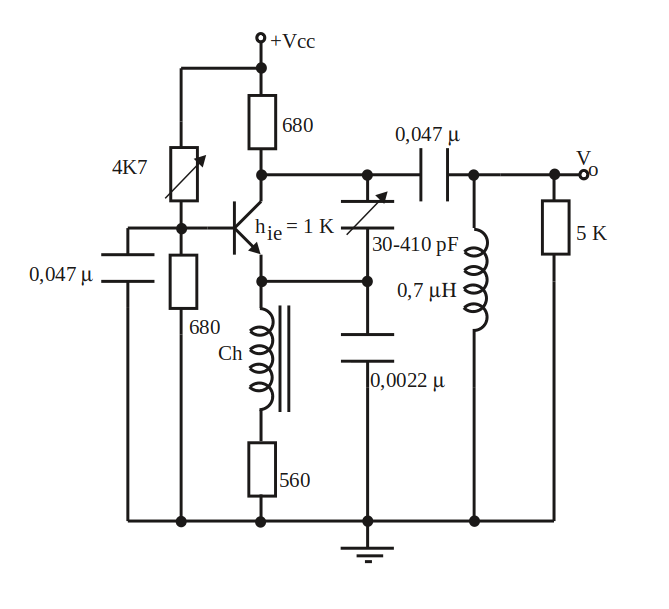
\includegraphics[width=0.8\linewidth]{figuras/oscila10.png}\\
	\caption{Ejercicio 10.}\label{oscila10}
\end{figure}


\textbf{Ejercicio 11}: Para el oscilador a cristal mostrado en la
figura \ref{oscila11}, hallar el valor de R para oscilación crítica,
la frecuencia exacta de oscilación, y la estabilidad en frecuencia
del circuito.

\begin{figure}
	\centering
	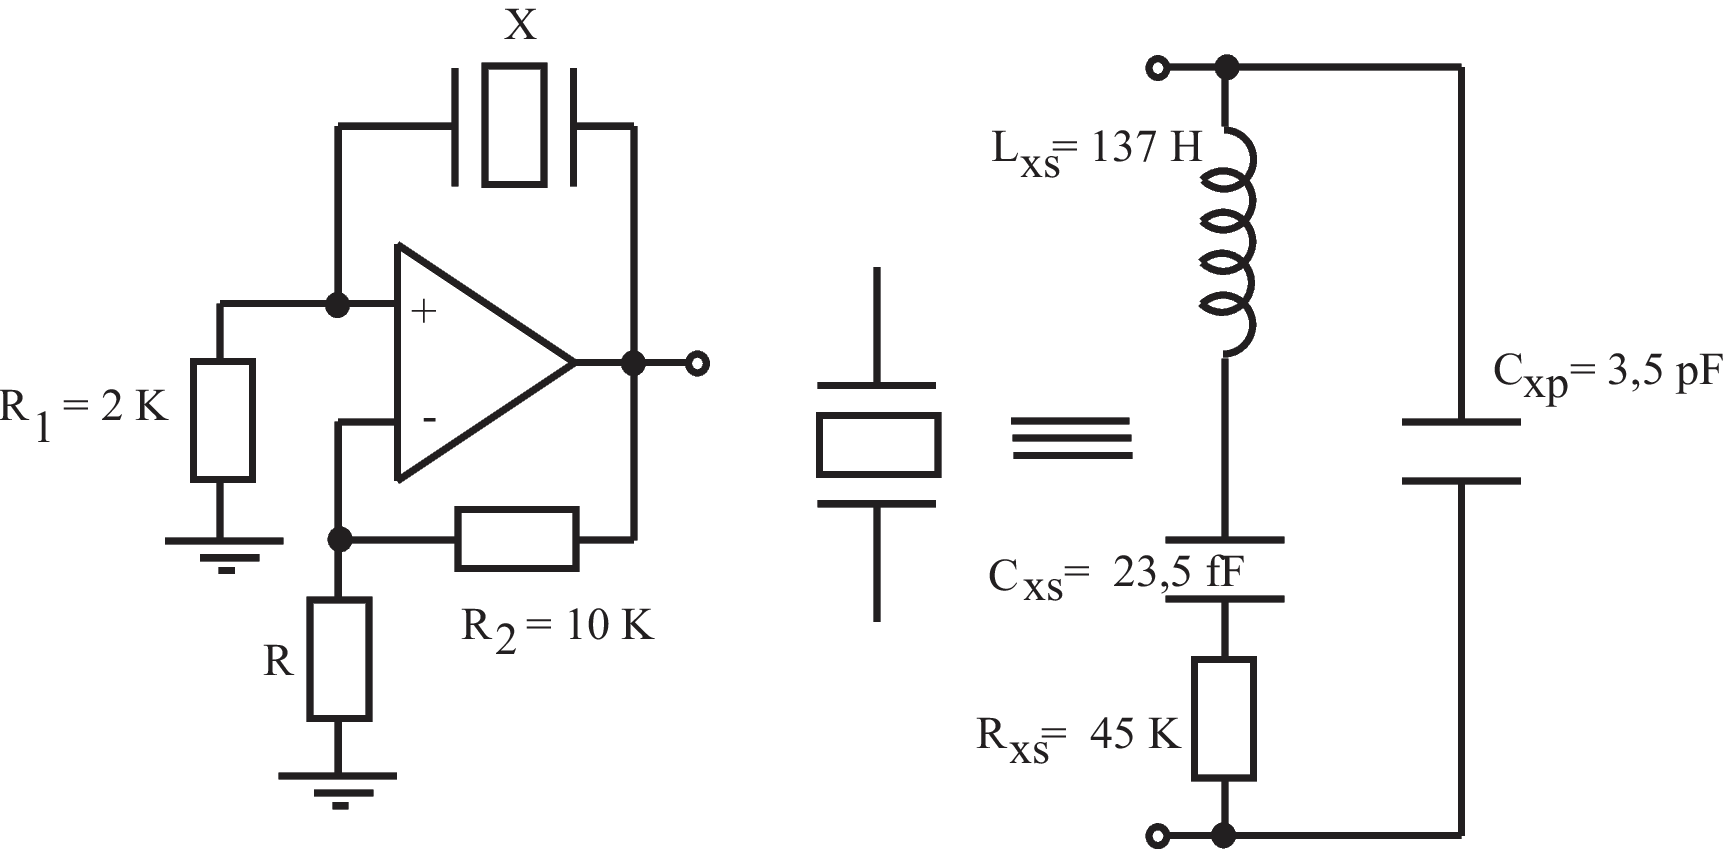
\includegraphics[width=0.8\linewidth]{figuras/oscila11.png}\\
	\caption{Ejercicio 11.}\label{oscila11}
\end{figure}



\textbf{Ejercicio 12}:  En el circuito de la figura \ref{oscila12},
calcular la frecuencia de oscilación e indicar si se cumple la
condición de amplitud.




\begin{figure}
	\centering
	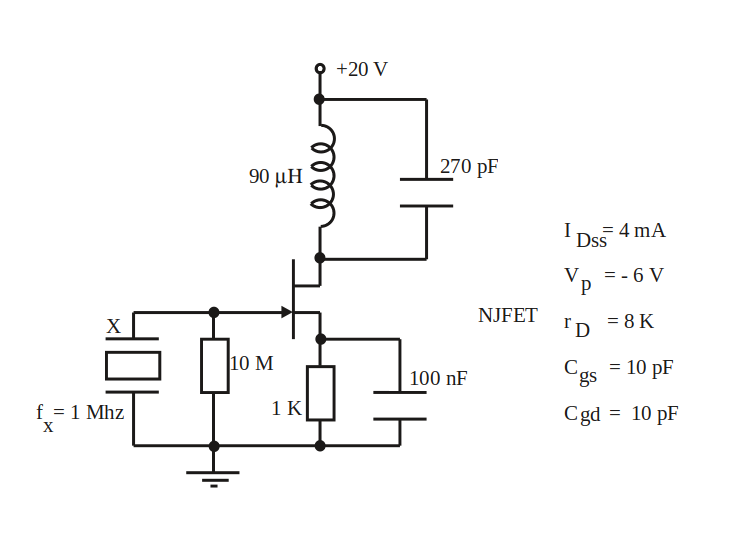
\includegraphics[width=0.8\linewidth]{figuras/oscila12.png}\\
	\caption{Ejercicio 12.}\label{oscila12}
\end{figure}

